\chapter{Dokumente}
\label{dokumente}
Ein Student mu� zu Beginn seines Studiums verschiedenen Dokumente in Original vorzeigen und Kopien abgeben. In dieser Karteikarte wird festgehalten, welche bereits vorgelegt wurden.
Abbildung \ref{Dokumente1} zeigt den Aufbau der Karteikarte \textsl{Dokumente}:
\begin{itemize}
	\item Liste \textsl{Noch nicht abgegeben}: In diesem Listenfeld werden alle m�glichen und noch nicht abgegebenen Dokumente aufgelistet.
	\item Liste \textsl{Abgegeben}: Auslistung aller abgegebenen Dokumente.
	\item Button \textsl{=>}: Die im linken Feld markierten Dokumente-Eintr�ge werden in die rechte Liste der abgegebenen Dokumente �bertragen.
	\item Button \textsl{<=}: Dieser Korrekturbutton verschiebt markierte Dokumente-Eintr�ge in die Liste der noch nicht abgegebenen Dokumente.
	\item Button \textsl{Filter}: Wird dieser Button gedr�ckt, werden in der Studentenliste oberhalb des Krateireiters \textsl{Dokumente} alle jene Studenten angezeigt, die Dokumente noch nicht abgegeben haben.
\end{itemize}
\begin{figure}
	\centering
	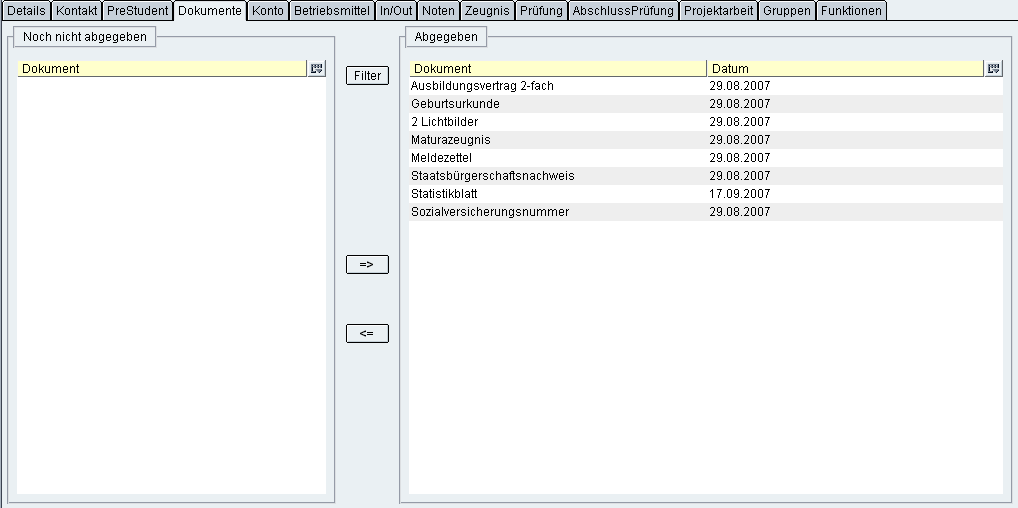
\includegraphics[width=0.75\textwidth]{FAS_Dokumente1.png}
	\caption{Die Karteikarte Dokumente}
	\label{Dokumente1}
\end{figure}